\vskip 1cm

\begin{center}
{\bf\LARGE 112neV parxkaraNa.}\\
\vskip .3cm
{\bf\large vuyxtakxrXma misharx vayxvahAravu.}\\
\end{center}

vuyxtakxma misharx gaNitagaLige $6$ vidhavAda sUtarxgaLanunx keLage vivarisalapxDuvavu. avugaLaLoLage yAva vidhadiMdalAdarU leKaKxgaLanunx mADi utatxragaLanunx tagiya bahudu.

\begin{verse}
udAharaNe, dara KaMDiV $1$kekx $44, 42, 33, 30$ rUpAyigaLa parxkArakekx $4$ bageV goVdhiyanunx karxyakekx  tegadu koMDu misharx mADi, A misharxdhAnayxvanunx $36$ rUpAyige $1$ KaMDiyaMte mAra beVkeMdu iCeYsidare, yAvAyxva darada goVdhiyanunx eSeTxSuTx KaMDigaLanunx tegadu koLaLx beVku, heVLu?
\end{verse}

\begin{figure}[H]
\centering
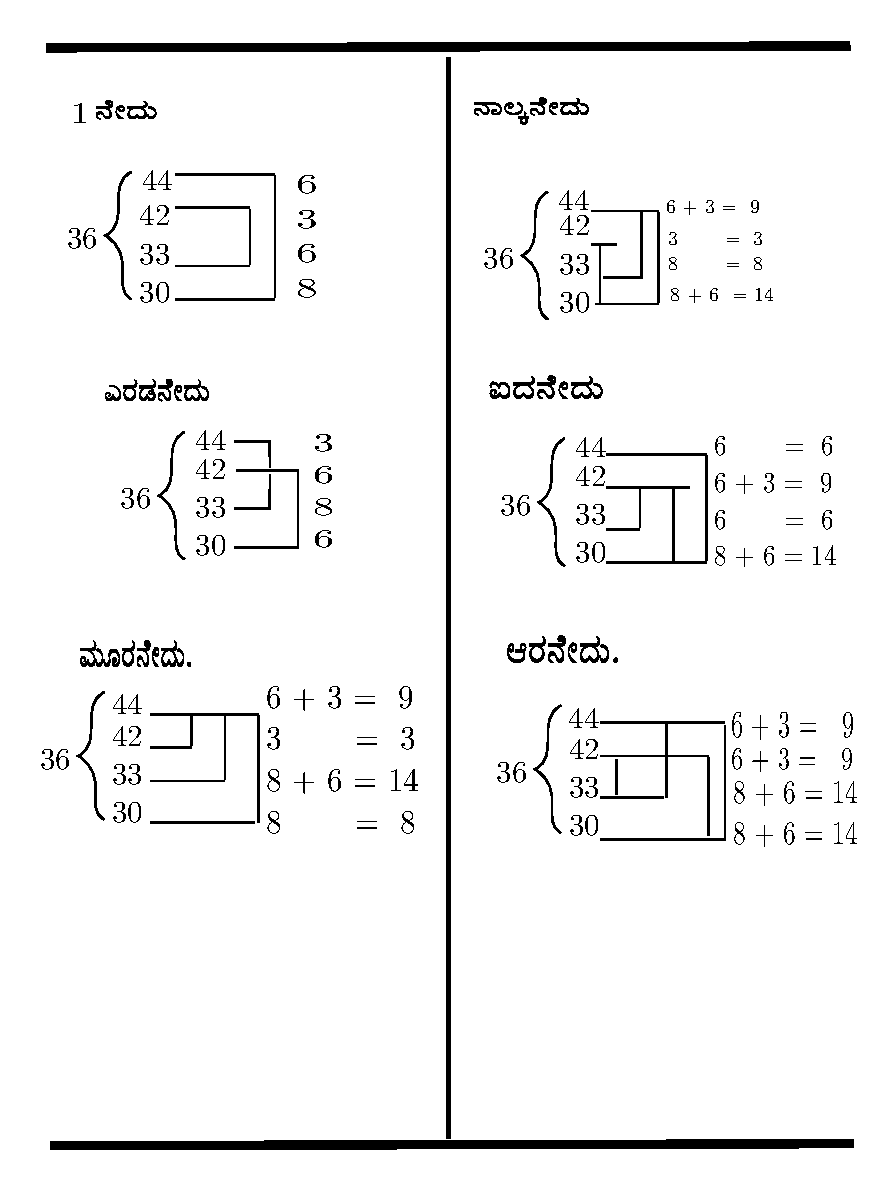
\includegraphics{7.eps}
\end{figure}


\begin{verse}
sU|| $1$neVdu. misharx bele $36$kUkx shudadhx bele $44$kUkx iruva vetAyxsa $8$nunx $30$ra muMdU, matUtx $36$kUkx $30$kUkx iruva vetAyxsa $6$nunx $44$ra muMdU, matutx $36$kUkx $33$kUkx iruva vetAyxsa $3$nunx $42$ra muMdU, $36$kUkx $42$kUkx iruva vetAyxsa $6$nunx $33$ra muMdU, baradu irutatxde eMtatxlU, avugaLeV AyAya darada KaMDi parxmANagaLeMtatxlU, muMde iruva $5$ riVtigaLanUnx avugaLa muMde baradiruva reVKegaLiMda Uhisa takakxdeMtalU tiLiya beVku.
\end{verse}

\begin{center}
{\bf\large udAharaNegaLu.}
\end{center}

\begin{enumerate}[\rm(1)]
\item $15, 17, 18, 22$ rUpAyigaLige toVlAdaMte iruva nAlukx begeV BaMgAravanunx tegadukoMDu karagi\-si $20$ rUpAyige toVlAdaMte $40$ tolA BaMgAravanunx tegadukoMDu mAra beVkeMdiCeCxYsidare, yAvAyxva daradudx eSeTxSuTx tegadukoLaLx beVku.
\end{enumerate}

\begin{figure}[H]
\centering
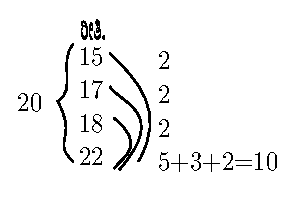
\includegraphics{8.eps}
\end{figure}

A parimANagaLanunx kUDisalu $16$ Agalu, hiVge terxYrAshiyanunx mADabeVku.

\qq\begin{tabular}{>{$}l<{$}>{$}l<{$}>{$}l<{$}>{$}l<{$}>{$}l<{$}>{$}c<{$}>{$}c<{$}l}
16 \text{kekx}& : & 40 & :: & ~~2 & = & ~5 & idu $15$rU. darada tolA.\\
16 & : & 40 & :: & ~~2 & = & ~5 & idu $17$rU. darada tolA.\\
16 & : & 40 & :: & ~~2 & = & ~5 & idu $18$rU. darada tolA.\\
16 & : & 40 & :: & 10 & = & 25 & idu $22$rU. darada tolA.\\
\cline{7-7}
&&&&&&40& aMtU nalavatutx.
\end{tabular}\\


$(2)$ dara gAyxla\char'366 $1$kekx SililxMgf, $5$ SililxMgf $6$ pa\char'366sf, matutx $6$ SililxMgf, I darada nAlukx bageV dArxkeSx rasavanunx misharx mADi, daragAyxla\char'366 $1$kekx $5$ SililxMgf $4$ pe\char'366sinaMte mAra beVkeMtalU, avugaLalilx $4$ SililxMgf daradudx mAtarx $3$ mUreV gAla\char'366 ira beVkeMtalU iCeCxYsidare, yAvAyxva daradudx eSeTxSuTx tegadukoLaLx beVku?

\begin{center}
{\bf riVti.}
\end{center}

daragaLige oTiTxge pe\char'366sfgaLanunx mADikoLaLxlu.

\begin{figure}[H]
\centering
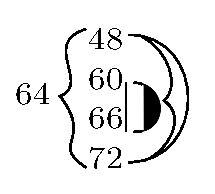
\includegraphics{9.eps}
\end{figure}

\qq\qq\begin{tabular}{>{$}c<{$}c>{$}c<{$}>{$}l<{$}>{$}l<{$}}
~8 & athavA & ~8+2 &= & 10\\
~2 & athavA & ~8 + 2 & = & 10\\
~4 & athavA & 16+4 & = & 20\\
16 & athavA & 16 + 4 & =& 20
\end{tabular}\\

idaralilx $4$ gAyxla\char'366 daradudx $8$ athavA $10$ gAyxla\char'366gaLu baMdirutatxve, 

AdadxriMda hiVge terxYrAshi mADa beVku. \qq\qq\qquad athavA\\

\begin{tabular}{>{$}l<{$}>{$}l<{$}>{$}l<{$}>{$}l<{$}>{$}c<{$}>{$}l<{$}>{$}c<{$}}8\text{kekx} & : & 3 & :: & ~8 & = & ~3\\
8 & : & 3 & :: & ~2 & = & ~\tfrac{3}{4}\\[3pt]
8 & : & 3 & :: & ~4 & = & 1\tfrac{1}{2}\\
8 & : & 3 & :: & 16 &= &  ~6\\
\end{tabular}
\qq\begin{tabular}{>{$}l<{$}>{$}l<{$}>{$}l<{$}>{$}l<{$}>{$}c<{$}>{$}l<{$}>{$}c<{$}}
10\text{kekx} & : & 3 :: & 10 & = & 3\\
10 & : & 3 :: & 10 & = & 3\\
10 & : & 3 :: & 20 & = & 6\\
10 & : & 3 :: & 20 & = & 6\\
\end{tabular}

\begin{center}
{\bf\large 128neV aBayx udAharaNe.}
\end{center}

\begin{enumerate}[\rm(1)]
\item obabx vAyxpAriyu $12, 10, 6, 4,$ rUpAyigaLige maNada darada dhAnayxgaLanunx tegadukoMDu berikeV mADi mAra beVkeMtalU adaralilx $4$ rUpAyi daradudx mAtarx $20$ maNagaLira beVkeMtalU, adaralilx $4$ rUpAyi daradudx mAtarx $20$ maNagaLira beVkeMtalU, tanige berike dhAraNeyu maNa $1$kekx $8$ rUpAyi biVLa beVkeMtalU iCeCxYsutAtxne. Agalu avanu yAvAyxva daradudx eSeTxSuTx maNagaLanunx tegadukoLaLx beVku?

\item obabx reYtana BUmige oTiTxge KaMDi $1$kekx $28$ rUpAyigaLu kaMdAya bididxruvavu. AdAgUyx avana BUmiyalilx dara KaMDi $1$kekx $63, 49, 35, 23, 12$ rUpAyigaLa daravuLaLx parxteyxVka BUmigaLidadxvu. Adare yAvAyxva darada BUmi eSeTxSuTx KaMDigaLidadxvu?

\item obabxnu $16, 18, 22,$ rUpAyigaLige KaMDiyaMte yiruva $3$ bageV kaDelxyanunx tegadukoMDu berasi, $20$ rUpAyige KaMDagadaMteV mAra beVkeMdu koVrutAtxne. Aga yAvAyxva daradudx eSeTxSuTx KaMDigaLanunx tegadukoLaLx beVku? 

\end{enumerate}

 
